
Pinpoint provides users with an interactive 3D scene in which electrophysiology trajectories can be explored within the anatomical context of the mouse brain (Fig. Xy). At the center of the 3D scene we render transparent 3D meshes for the major brain structures in the mouse Common Coordinate Framework (CCF) \citep{wang2020allen}. Individual brain regions can be highlighted through a search menu. 3D models of Neuropixels probes \citep{jun2017fully} can be added to the scene and moved through intuitive click+drag (or keyboard) interactions. Pinpoint provides feedback on the brain areas that each probe is passing through via a ``probe panel'' and an ``in-plane slice''. The view has space to render 16 probe shanks at a time, supporting either 16 individual 1-shank Neuropixels probes or four 4-shank probes. Additional features include the ability to snap probes to brain regions, design plans for craniotomy surgeries, detect collisions between probes and between probes and rig hardware, save experimental plans, and automate experiments. By running in both web browsers and as a standalone application, Pinpoint lowers the barrier to experimental planning and disconnects the need for expert anatomical knowledge of the brain from the technical skill required to perform complex simultaneous multi-probe recordings. 

\begin{figure}
\centering

\includegraphics[keepaspectratio,width=0.4\textwidth]{figures/figure-1.pdf}
\caption[mini-caption]{Title. Caption}
\label{fig:pinpoint_overview}
\end{figure}

\subsection{Planning an insertion in 3D space}

In the following sections we describe the features in Pinpoint that enable users to plan a trajectory. These steps can also be followed in online \href{https://virtualbrainlab.org/02_traj_planner/02_tp_tutorial.html}{video tutorials}. 

To target particular brain regions users can snap probes to the center of regions and then perform further manual alignment to optimize their trajectory in 3D space. By default, Pinpoint loads the top-level of the CCF hierarchy and displays these brain regions as transparent meshes. To target more specific regions or layers, users can search for these in the search bar (Figure). Clicking on a region highlights the 3D mesh in the scene using an opaque texture and pressing the ``snap'' button moves the probe tip to the center of the 3D mesh. Once the probe tip is positioned, users can use either click+drag controls with their mouse, or keyboard presses to optimize the alignment. To use the keyboard controls, users press the keys corresponding to the different axis directions: anterior-posterior: W and S, left-right A and D, dorsal-ventral: E and Q. Users can also rotate probes: pitch: R and F, yaw: 1 and 3, spin: , and . . To move the probe along its depth axis users can press Z or X. Each of these keyboard presses moves the probe tip by 10 um along that axis. Holding shift increases the step size to 100 um while holding control reduces it to 1 um. To use the click+drag controls, users click the left mouse button on the 3D model of the probe and then press any of the axis keys (e.g. W or S for anterior-posterior). Dragging the mouse along the corresponding axis will then move the probe continuously.

% stereo coordinates
After planning a recording, Pinpoint provides users with the stereotaxic coordinates and angles needed to reproduce the insertion in the live mouse brain. Pinpoint defines an insertion using the entry coordinate on the surface of the brain, defined by its (AP, ML, DV) position relative to Bregma (??). Probe angles are defined as (Pitch, Yaw, Spin), where pitch is the angle off of the horizontal plane, yaw is the rotation of the probe around the Z (up) axis, and spin is the rotation of the probe around its own axis. To perform a recording, users set up their probe according to the specified angles, zero their stereotax with the probe tip at Bregma, and move the probe to the entry coordinate. Once at the entry coordinate, the target brain area is reached by moving only along the depth axis.

\begin{figure}
\centering
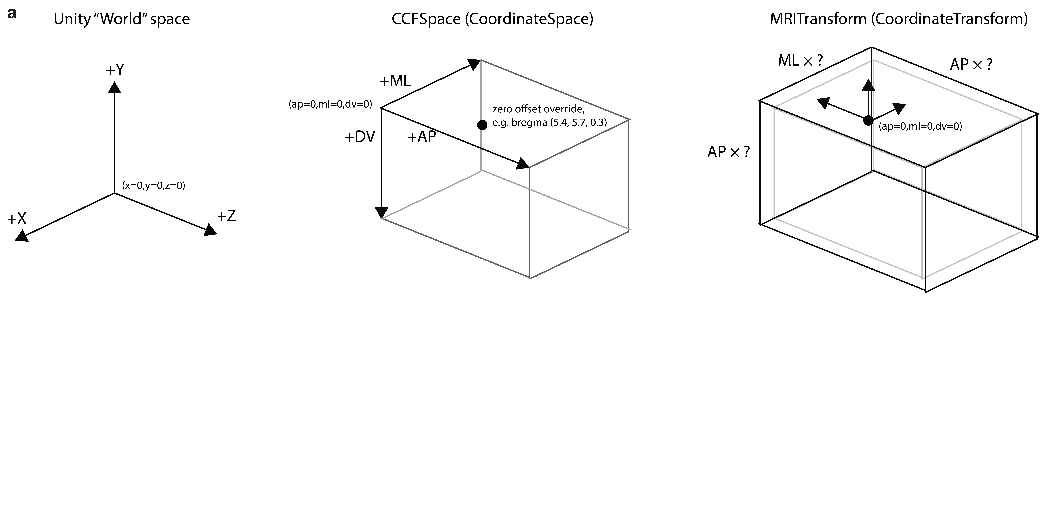
\includegraphics[keepaspectratio,width=0.4\textwidth]{figures/figure-2.pdf}
\caption[mini-caption]{Title. Caption}
\label{fig:coordinate_spaces}
\end{figure}

% coordinate spaces
When using Pinpoint, users can choose to plan their trajectories in raw CCF space or in a deformation of CCF to better match the live mouse brain. The CCF was defined using perfused brains, which are warped and stretched compared to the live brain. The transformed spaces were defined from anatomical MRI images that were aligned to the CCF, but in theory provide a better estimate of the live mouse brain depending on the age and strain. We provide a variety of transformation options as well as options to scale the transformed space according to the Bregma-Lambda distance.

\begin{figure}
\centering
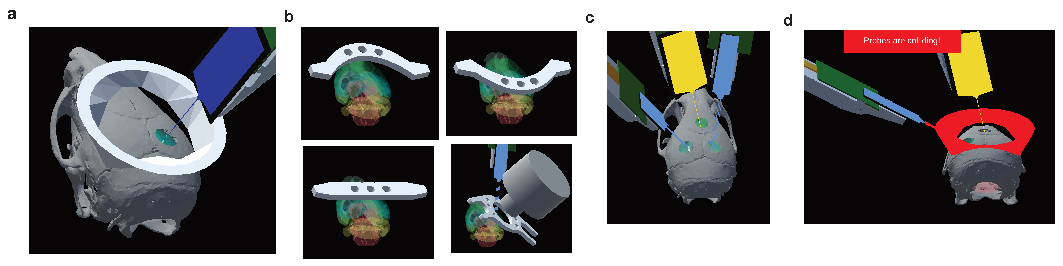
\includegraphics[keepaspectratio,width=0.4\textwidth]{figures/figure-3.pdf}
\caption[mini-caption]{Title. Caption}
\label{fig:rig_hardware}
\end{figure}

% avoiding rig hardware
The interactive 3D scene in Pinpoint provides a number of affordances that help with planning trajectories alongside complex surgical and hardware constraints. Alongside the 3D probe models, Pinpoint can display a skull model and allow users to explore possible craniotomies for surgery (Fig. Xy). Another example, simultaneous recordings with both 2-photon calcium imaging and electrophysiology probes, imaging hardware can limit the angles at which probes can be inserted.

% saving experiments

\subsection{Automation}

\begin{figure}
\centering
\includegraphics[keepaspectratio,width=0.4\textwidth]{figures/figure-4.pdf}
\caption[mini-caption]{Title. Caption}
\label{fig:automation}
\end{figure}

% live echoing
In addition to the trajectory planning features, we also designed Pinpoint to act as a link to hardware manipulators, both to show the live position of probes in the brain and to enable automated insertion of probes. In parallel to Pinpoint we have developed a Python package ``ephys-link'' that handles communication with hardware manipulators (currently, Sensapex uMP-4 and New Scale ??). Ephys-link automatically detects and communicates with connected manipulators and exposes a WebSocket connection for communicating with Pinpoint. Once connected, users have to ensure that their probe type and angles match the live probe and set a reference point so that Pinpoint can compute the relative position of the live probe in the 3D scene. After linking, probe movements are echoed in the scene allowing users to visualize their probe position live in the mouse brain. 

% automated insertions
When connected to the ephys-link package, Pinpoint can also perform some parts of the insertion process automatically. We have developed automation tools to accelerate the process of handling large numbers of probes, in particular to enable users to perform 4+ multi-probe recordings in an efficient and safe manner. To do this, we have built into Pinpoint a standard sequence for performing multi-probe insertions: first, users set up the Pinpoint scene to have the 3D models of all probes (Fig. Xy), second, they link these probes to the hardware manipulators and choose the target insertions (Fig. Xy), third, they zero all of the probes at Bregma individually, and finally, they allow the insertion sequence to run. The sequence moves probes first to their insertion coordinate, then allows the user to punch through the dura, and finally drives the probes to the appropriate depth. In the future, we hope to enable complete automation through the use of external cameras to detect probe positions, craniotomy locations, blood vessels, and probe bending during insertion. 